\input{preamble}
\input{format}
\input{commands}

\begin{document}

\begin{Large}
    \textsf{\textbf{Homework 7}}
    
    \textbf{Circle Finding Algorithm}
\end{Large}

\vspace{1ex}

\textsf{\textbf{Student:}} \text{Yuanyuan Zhao, 2300013077, School of EECS}, \href{mailto:your.email@hotmail.com}{\texttt{zhaoyuanyuan@stu.pku.edu.cn}}\\
\textsf{\textbf{Lecturer:}} \text{Yisong Chen}
% \href{mailto:your.email@hotmail.com}
% {\texttt{chenyisong@pku.edu.cn}}\\


\vspace{2ex}


\begin{problem}{Circle Finding Algorithm Design}{algo}
    I implemented 2 algorithms to find circles. In algorithm1.mlx, I attempted to design a customized algorithm, which consists of Canny edge detection, curvature-based arc segmentation, RANSAC-inspired circle fitting and metal reflectance validation. However, it turned out unsatisfactory, so I moved on to implement a Hough Transform version with something novel in algorithm2.mlx, which achieves a good performance.

\begin{enumerate}[(a)]
    \item \textbf{Customized Algorithm}
    \begin{enumerate}[label = (\roman*)]
        \item Preprocessing (Canny edge detection)
        \begin{verbatim}
        if size(img, 3) == 3
            grayImg = rgb2gray(img);
        else
            grayImg = img;
        end
        edges = edge(grayImg, 'canny', p.Results.EdgeThreshold);
        \end{verbatim}
        

        \item Arc Detection
        $$
        \kappa_i=\frac{\Vert (P_{i-k}-P_i)\times (P_{i+k}-P_i)\Vert}{\Vert P_{i-k}-P_i\Vert ^3}
        $$
        \begin{verbatim}
        function curvature = computeCurvature(contour)
            n = size(contour, 1);
            curvature = zeros(n, 1);
            for i = 1:n
                prev = contour(max(1, i-5), :);
                next = contour(min(n, i+5), :);
                vec1 = contour(i,:) - prev;
                vec2 = next - contour(i,:);
                curvature(i) = abs(vec1(1)*vec2(2) - vec1(2)*vec2(1)); 
            end
            curvature = curvature / max(curvature); 
        end
        \end{verbatim}

        \item Geometric Verification
        \begin{verbatim}
        x = pts(:,1); y = pts(:,2);
        A = 2 * [x(2)-x(1), y(2)-y(1); x(3)-x(1), y(3)-y(1)];
        b = [x(2)^2 - x(1)^2 + y(2)^2 - y(1)^2; 
             x(3)^2 - x(1)^2 + y(3)^2 - y(1)^2];
        center = (pinv(A) * b)'; 
        radius = sqrt((x(1)-center(1))^2 + (y(1)-center(2))^2);
        \end{verbatim}
    \end{enumerate}

    
    \item \textbf{Hough Transform Algorithm}
        \begin{enumerate}[label = (\roman*)]
            \item Gauss Smoothing and Canny Edge Detection
            
            At first Canny detection wad deployed directly without any smoothing, and the results turned out of great redundancy, so I add a gauss filter before edge detection.
            \begin{verbatim}
            gaussFilter = fspecial('gaussian', filterSize, sigma);
            smoothImg = imfilter(grayImg, gaussFilter, 'replicate');
            edges = edge(smoothImg, 'canny');
            \end{verbatim}
            \item Hough Transform

             \begin{verbatim}
            [y, x] = find(edges);
            for i = 1:length(x)
                for rIdx = 1:length(radiusRange)
                    r = radiusRange(rIdx);
                    for theta = 0:360
                        thetaRad = deg2rad(theta);
                        a = round(x(i) - r * cos(thetaRad));
                        b = round(y(i) - r * sin(thetaRad));
                        if a > 0 && a <= size(edges, 2) 
                                    && b > 0 
                                    && b <= size(edges, 1)
                            accumulator(b, a, rIdx) = 
                                    accumulator(b, a, rIdx) + 1;
                        end
                    end
                end
            end
            \end{verbatim}
            \item Find Local Maximum
            \begin{verbatim}
            for rIdx = 1:length(radiusRange)
                [b, a] = find(accumulator(:,:,rIdx) > 
                            0.5 * max(accumulator(:))); 
                for i = 1:length(a)
                    circles = [circles; a(i), b(i), radiusRange(rIdx)];
                end
            end
            \end{verbatim}
            \item Remove Redundancy
            \begin{verbatim}
            if distance < distanceThreshold 
                        && radiusDiff < radiusThreshold
                if circles(i, 3) < circles(j, 3)
                    toDelete(i) = true;
                else
                    toDelete(j) = true;
                end
            end
            \end{verbatim}
    \end{enumerate}
    
\end{enumerate}
\end{problem}

\begin{figure}[htbp]
    \centering 
    \begin{minipage}{0.8\textwidth} 
        \centering 
        
        \begin{subfigure}[b]{0.45\linewidth} 
            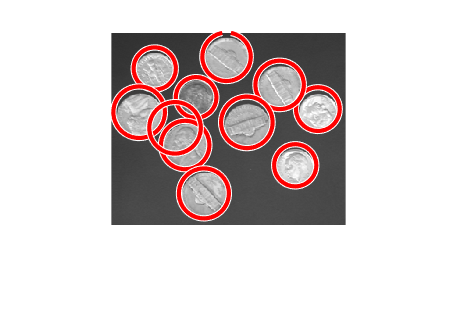
\includegraphics[width=\linewidth]{images/coins_result.png}
            \caption{minRadius=25, maxRadius=35}
        \end{subfigure}
        \hfill
        \begin{subfigure}[b]{0.45\linewidth}
            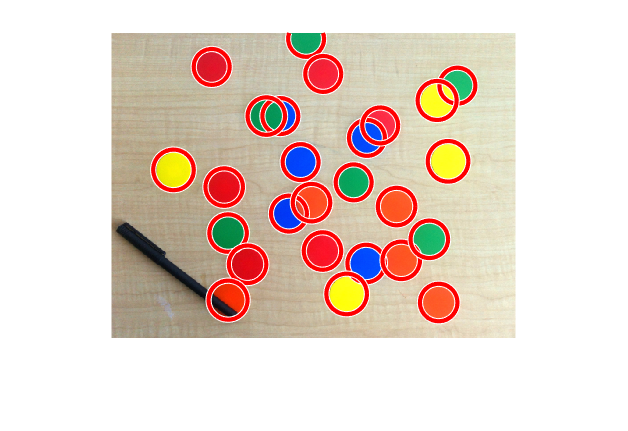
\includegraphics[width=\linewidth]{images/coloredChips_result.png}
            \caption{minRadius=15, maxRadius=30}
        \end{subfigure}

        \vspace{0.5cm}
        \begin{subfigure}[b]{0.45\linewidth}
            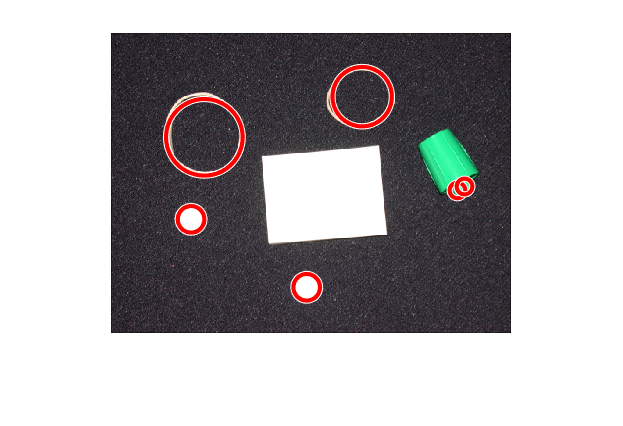
\includegraphics[width=\linewidth]{images/pillsetc_result.png}
            \caption{minRadius=10, maxRadius=50}
        \end{subfigure}
        \hfill
        \begin{subfigure}[b]{0.45\linewidth}
            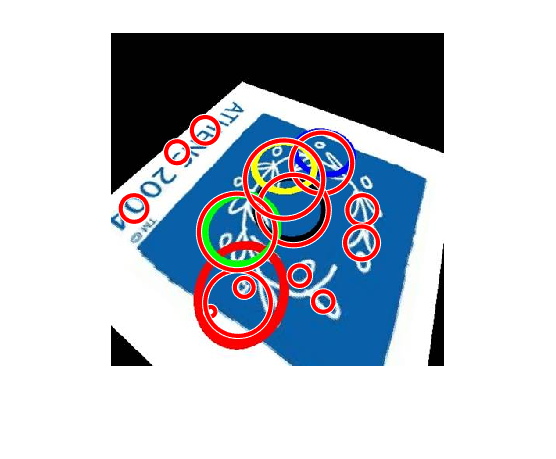
\includegraphics[width=\linewidth]{images/olympic_result.png}
            \caption{minRadius=5, maxRadius=50}
        \end{subfigure}

        \caption{myFindCircle with different radius parameters}
        \label{fig:Colmar}
    \end{minipage}
\end{figure}



\begin{problem}{Result Analysis}{result}

    The results are satisfactory to a large extent, but there're still some problems. To be specific, in coin.png, there is one redundant circle, and when I adjust the parameter of removeOverlappingCircles function trying to remove it, the correct circle disappears. And in olympic.jpg, the characters and patterns trigger some false circles. Those results show that the curvature algorithm is too sensitive to noise and the selection of redundancy is not perfectly accurate. Thus, the algorithm may not be suitable for some complicated scenario.

    In addition, manual adjustment of minRadius and maxRadius is needed, making it inapplicable when the radius of target circles are totally unknown.

\end{problem}





% =================================================

% \newpage

% \vfill

\end{document}